\documentclass[10pt,a4paper]{article}
\usepackage[UTF8]{ctex}
\usepackage{geometry}
\geometry{
    top=15mm,
    bottom=15mm,
    left=14mm,
    right=14mm,
    headheight=14pt,
    footskip=10mm
}
\usepackage{pdfpages}
\usepackage{fancyhdr}
\usepackage{tikz}

\pagestyle{fancy}
\fancyhf{}
\fancyhead[C]{\small LingXiAgent 本地自主智能体软件 V1.0}
\renewcommand{\headrulewidth}{0.4pt}
\renewcommand{\footrulewidth}{0pt}

% 覆盖原底端长页码，统一渲染软著标准交存页码：第 X 页 / 共 60 页
\fancyfoot[C]{%
  \begin{tikzpicture}[remember picture,overlay]
    \node[fill=white,minimum width=65mm,minimum height=9mm] at (0,0) {};
    \node at (0,0) {\small 第 \thepage\ 页 / 共 60 页};
  \end{tikzpicture}%
}

\begin{document}
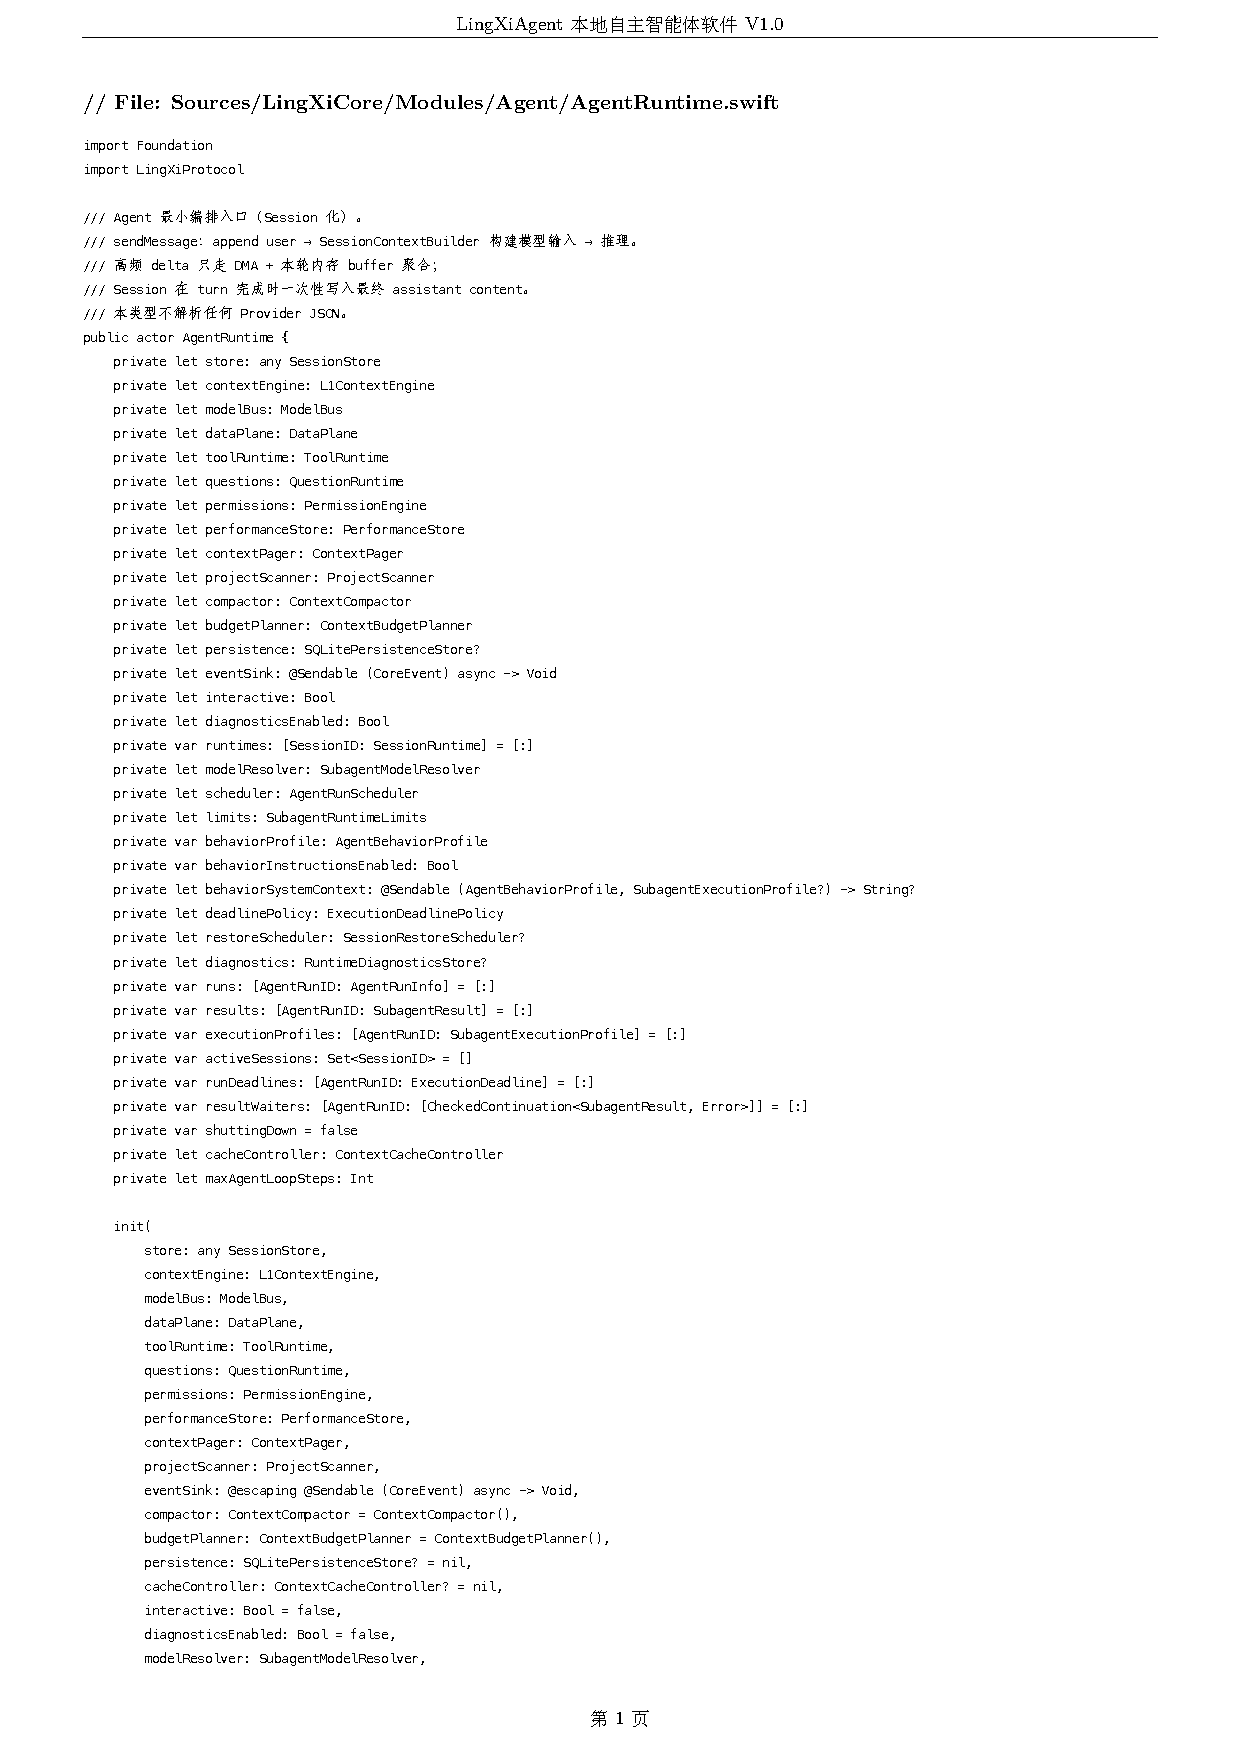
\includepdf[pages={1-30,276-305},pagecommand={\thispagestyle{fancy}}]{LingXiAgent-V1.0-source-full.pdf}
\end{document}
